\subsection*{Problema 06}

En este problema se calculará la integral indefinida:

\begin{equation*}
\int \dfrac{\sin x \, dx}{1 + \cos x}
\end{equation*}

\textbf{Solución:}

Para resolver esta integral, utilizaremos el método de sustitución (cambio de variable). 
Primero, definimos una nueva variable $u$ igual al denominador de la función integrada:

\begin{equation*}
u = 1 + \cos x
\end{equation*}

A continuación, calculamos la diferencial $du$ derivando $u$ respecto a $x$:

\begin{align*}
du &= \dfrac{d}{dx}(1 + \cos x) \, dx \\
du &= -\sin x \, dx
\end{align*}

Despejamos el término que contiene al seno para que coincida con el numerador de nuestra integral:

\begin{equation*}
-\,du = \sin x \, dx
\end{equation*}

Sustituimos $u$ y $du$ en la integral original. 
Reemplazamos $\sin x \, dx$ por $-\,du$ y $1 + \cos x$ por $u$:

\begin{align*}
\int \dfrac{\sin x \, dx}{1 + \cos x} &= \int \dfrac{-\,du}{u} \\
&= -\int \dfrac{1}{u} \, du
\end{align*}

Ahora, resolvemos la integral básica resultante, la cual corresponde a la función logaritmo natural:

\begin{equation*}
-\int \dfrac{1}{u} \, du = -\ln|u| + C
\end{equation*}

Finalmente, regresamos a la variable original $x$ sustituyendo $u = 1 + \cos x$:

\begin{equation*}
-\ln|1 + \cos x| + C
\end{equation*}

Por lo tanto, el resultado de la integral es:

\begin{equation*}
\int \dfrac{\sin x \, dx}{1 + \cos x} = -\ln|1 + \cos x| + C
\end{equation*}

\begin{figure}[H]
	\centering
	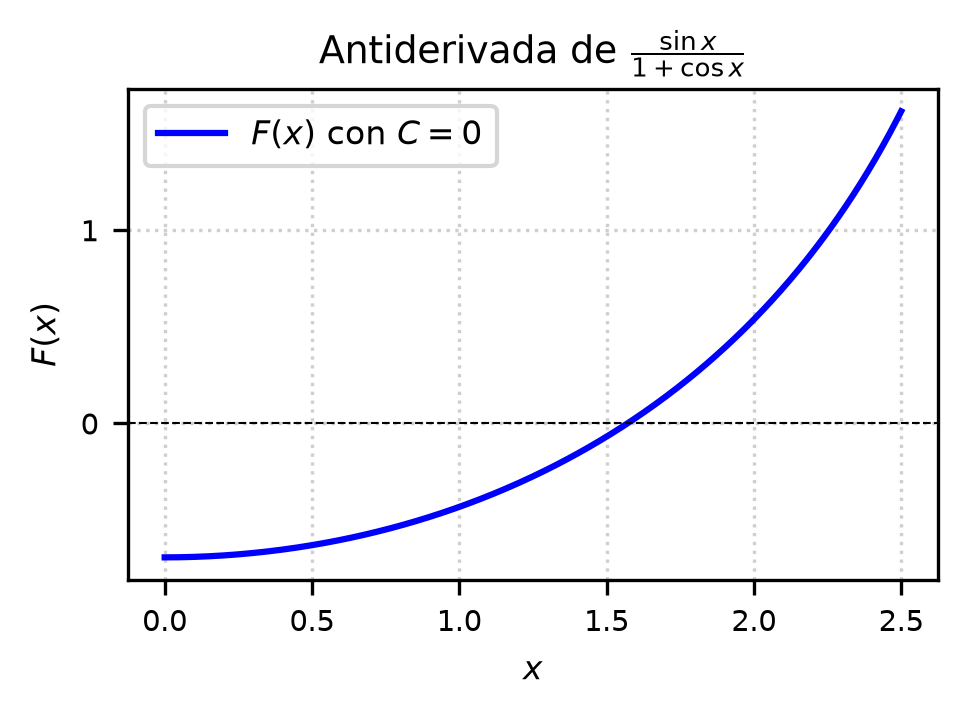
\includegraphics[width=\columnwidth]{semana_04/graficas/SEM04_P06_grafica.png}
	\caption{Representación gráfica de $f(x)$ y su antiderivada $F(x)$ evaluada para la constante de integración $C = 0$ (Problema 06).}
	\label{fig:problema06}
\end{figure}
